% El tipo de regla de negocio (tercer parámetro del entorno 'BusinessRule') se describe en la siguiente tabla:
%---------------------------------------------------------------------------------------------------------------,
% TIPOS		|		DEFINICION		|	EJEMPLO						|
%---------------|---------------------------------------|-------------------------------------------------------|
% Habilitador   | La sentencia habilita o restringe 	| * Se pueden recibir solicitudes del tipo A, B y C.	|
%		| hacer algo o  una funcionalidad.	| * Se permite hacer algo si se tiene el estado X.	|
%---------------|---------------------------------------|-------------------------------------------------------|
% Cronometrado	| Se permite de manera controlada 	| * Se permiten hasta dos solicitudes del tipo D	| 
%		| por un contador.			|   por persona.					|
% 		|					| * El acceso al sistema se permite si no se tiene 	|
%  		|					|   más de X número de intentos fallidos.		|
%---------------|---------------------------------------|-------------------------------------------------------|
% Ejecutivo	| Autorizado por un superior, un perfil | * Se permite registrar extemporaneamente si lo 	|
%		| particular debe autorizar.		|   autoriza X.						|
%---------------|---------------------------------------|-------------------------------------------------------|
% Derivación	| Son de cálculo e inferencia, 		| * Un alumno irregular es aquel que tiene las 		|
%		| es un cálculo o conclusión derivados 	|   siguientes cacteristicas: A, B, C. 			|
%		| de un conjunto de datos. Puede ser una| * El formato de un correo o CURP.			|
%		| fórmula que dice cómo calcular algo 	|							|
%		| o el formato de un dato.		|							|
%---------------|---------------------------------------|-------------------------------------------------------|
% Restricción	| Restringe una funcionalidad o relación| * Traslape de fechas o periodos empalmados.		|
% 		| entre dos o mas objetos.		|							|
%  		|					|							|
%---------------------------------------------------------------------------------------------------------------'

% No editar las reglas cuyo estatus es APROBADO.

\section{Reglas de negocio}
%%------------------------------------------------------------------------------------------------------------------
%============================== RN1 =================================
\begin{BusinessRule}{RN1}{Campos obligatorios}
	{Restricción}
	{Controla la operación}
	\BRitem{Versión}{1.0}
	\BRitem{Autor}{Adrian Flores Torres}
	\BRitem{Estatus}{Terminada}
	\BRitem{Descripción}{La información que se proporcione en los campos marcados como obligatorios debe ser ingresada para poder continuar con la operación requerida.}
	\BRitem{Referenciado por}{
	\cdtIdRef{CUA1.1}{Iniciar sesión}, \cdtIdRef{CUA1.2}{Registro de cuenta}
	}
	
\end{BusinessRule}

%============================== RN2 =================================
\begin{BusinessRule}{RN2}{Formato válido para un correo electrónico}
	{Restricción}
	{Controla la operación}
	\BRitem{Versión}{1.0}
	\BRitem{Autor}{Adrian Flores Torres}
	\BRitem{Estatus}{Terminada}
	\BRitem{Descripción}{
	Para que un correo electrónico se considere válido debe cumplir con la siguiente expresión regular:\\
		\(
		\wedge [ \_ a - z 0 - 9 - ] + ( . [\ _ a - z 0 - 9 - ] + ) * @ [ a - z 0 - 9 - ] + ( . [ a - z 0 - 9 - ] + ) * ( . [ a - z ] \{ 2 , 4 \} )\$ 
		\)
	}
	\BRitem{Referenciado por}{
		\cdtIdRef{CUA1.1}{Iniciar sesión}, \cdtIdRef{CUA1.2}{Registro de cuenta}
	}
	
\end{BusinessRule}

%============================== RN3 =================================
\begin{BusinessRule}{RN3}{Numero de intentos para inicio de sesión}
	{Restricción}
	{Controla la operación}
	\BRitem{Versión}{1.0}
	\BRitem{Autor}{Adrian Flores Torres}
	\BRitem{Estatus}{Terminada}
	\BRitem{Descripción}{El usuario solo tendrá 3 intentos para poder iniciar sesión, de lo contrario la cuenta se bloqueará por 5 minutos. Cada que el usuario  inicie sesión el contador que controla el número de intentos se reiniciará a 0.}
	\BRitem{Referenciado por}{
		\cdtIdRef{CUA1.1}{Iniciar sesión}
	}
	
\end{BusinessRule}


%============================== RN4 =================================
\begin{BusinessRule}{RN4}{Información Correcta}
	{Restricción}
	{Controla la operación}
	\BRitem{Versión}{1.0}
	\BRitem{Autor}{Adrian Flores Torres}
	\BRitem{Estatus}{Terminada}
	\BRitem{Descripción}{La información que se proporcione en los campos debe cumplir con lo estipulado en el modelo de información.}
	\BRitem{Referenciado por}{
		\cdtIdRef{CUA1.1}{Iniciar sesión}
	}
	
\end{BusinessRule}

\begin{BusinessRule}{RN5}{Unicidad de Elementos}
	{Derivación}
	{Controla la operación}
	\BRitem{Versión}{1.0}
	\BRitem{Autor}{Adrian Flores Torres}
	\BRitem{Estatus}{Edición}
	\BRitem{Descripción}{Un elemento no se puede duplicar en todo el sistema, ni registrar más de una ocasión. La unicidad se determinará con base en la siguiente lista:
		\\ 
		\begin{enumerate}
			\item Cuenta:
			\begin{itemize}
				\item Correo electrónico
			\end{itemize}
			
		\end{enumerate}
		
		Las actividades antes mencionadas, son las principales que utilizan esta regla de negocio. 
	}
	
	\BRitem{Referenciado por}{
		\cdtIdRef{CUA1.2}{Registro de cuenta}
	
}
\end{BusinessRule}

%============================== RN6 =================================
\begin{BusinessRule}{RN6}{Formato de contraseña}
	{Restricción}
	{Controla la operación}
	\BRitem{Versión}{1.0}
	\BRitem{Autor}{Adrian Flores Torres}
	\BRitem{Estatus}{Terminada}
	\BRitem{Descripción}{Por la seguridad de los usuarios de In-Help, las contraseñas deben cumplir con las siguientes condiciones:
	\begin{itemize}
		\item Tener una longitud mínima de 8 caracteres.
		\item Contar con por lo menos un número.
	\end{itemize}	
}
	\BRitem{Referenciado por}{
		\cdtIdRef{CUA1.2}{Registro de cuenta}
	}
	
\end{BusinessRule}


%============================== RN6 =================================
\begin{BusinessRule}{RN7}{Fecha de nacimiento válida}
	{Restricción}
	{Controla la operación}
	\BRitem{Versión}{1.0}
	\BRitem{Autor}{Adrian Flores Torres}
	\BRitem{Estatus}{Terminada}
	\BRitem{Descripción}{Una fecha de nacimiento válida deberá cumplir con la siguiente condición:\\
		\begin{center}
			$Fecha_{Nacimiento}  < 01/01/2008$
		\end{center}
	Donde: 
	\begin{itemize}
		\item $Fecha_{Nacimiento} :$ Es la fecha de nacimiento que el usuario esta registrando.
	\end{itemize}
	}
	\BRitem{Referenciado por}{
		\cdtIdRef{CUA1.2}{Registro de cuenta}
	}
	
\end{BusinessRule}





\newpage
\section{Maquinas de Estados}

\hypertarget{cv:Cuenta}{\section{Modelo del ciclo de vida de una cuenta}}

La cuenta de un usuario puede pasar por una serie de etapas o 'estados' en la aplicación. El estado en el que se encuentre dicha materia controlará las acciones que puede o no realizar el actor. Los estados y transiciones posibles se muestran en la figura \ref{fig:maq:cuenta} y se describen a continuación.\\

\begin{figure}[htbp!]
	\centering
	\fbox{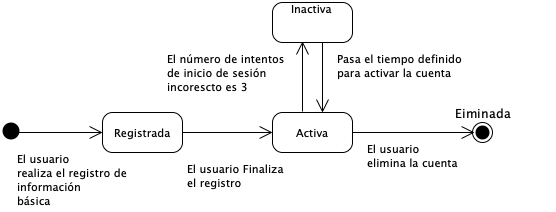
\includegraphics[width=\textwidth]{images/MaquinasEstado/MaquinaEstadosCuenta.png}}
	\caption{Modelo del ciclo de vida de una cuenta.}
	\label{fig:maq:cuenta}
\end{figure}

\noindent \textbf{Registrada:} Este es el estado inicial de una cuenta, cuando un usuario registra la información básica de la cuenta tiene dicho estado. Este estado es el inicio de la transición hacia el estado:
\begin{itemize}
	
	\item \textbf{Activa:} Pasa a este estado cuando el usuario termina de registrar la información complementaria de la cuenta.
	
\end{itemize}

\noindent \textbf{Activa:} En este estado el usuario ya finalizo el registro de la cuenta, registrando datos de contactos y de vehículos.Este estado tiene transición hacia los estados :
\begin{itemize}
	
	\item \textbf{Inactiva:} Pasa a este estado cuando el usuario intento ingresar a su cuenta y tuvo 3 intentos fallidos.
	\item \textbf{Eliminada:} Pasa a este estado cuando el usuario elimina la cuenta. 
\end{itemize}

\noindent \textbf{Inactiva:} Se encuentra en este estado cuando el usuario intento ingresar a su cuenta y el usuario era válido pero la contraseña la ingresó incorrectamente 3 veces. Este estado es el inicio de la transición hacia el estado:
\begin{itemize}
	
	\item \textbf{Activa:} Pasa a este estado cuando el temporizador de cuenta bloqueada llega al tiempo especificado.
	
\end{itemize}

\noindent \textbf{Eliminada:} Se encuentra en este estado una vez que el usuario elimina la cuenta. Este estado es es un estado final por lo que no genera transiciones a otro estado.
